% !TEX TS-program = pdflatex
% !TEX encoding = UTF-8 Unicode

% This is a simple template for a LaTeX document using the "article" class.
% See "book", "report", "letter" for other types of document.

\documentclass[11pt]{article} % use larger type; default would be 10pt

\usepackage[utf8]{inputenc} % set input encoding (not needed with XeLaTeX)

%%% Examples of Article customizations
% These packages are optional, depending whether you want the features they provide.
% See the LaTeX Companion or other references for full information.

%%% PAGE DIMENSIONS
\usepackage[top=2.1cm, bottom=2.1cm, left=2.1cm, right=2.1cm]{geometry}
\geometry{a4paper} % or letterpaper (US) or a5paper or....
% \geometry{margins=2in} % for example, change the margins to 2 inches all round
% \geometry{landscape} % set up the page for landscape
%   read geometry.pdf for detailed page layout information

%%% Line Spacing
\usepackage{setspace}
\onehalfspacing

\usepackage{sidecap}

\usepackage{graphicx} % support the \includegraphics command and options

% \usepackage[parfill]{parskip} % Activate to begin paragraphs with an empty line rather than an indent

%%% PACKAGES
\usepackage{booktabs} % for much better looking tables
\usepackage{array} % for better arrays (eg matrices) in maths
\usepackage{verbatim} % adds environment for commenting out blocks of text & for better verbatim
\usepackage{subfig} % make it possible to include more than one captioned figure/table in a single float
\usepackage{amsmath, amssymb, amsthm, lastpage}
% These packages are all incorporated in the memoir class to one degree or another...
\usepackage{url}

%%% HEADERS & FOOTERS
\usepackage{fancyhdr} % This should be set AFTER setting up the page geometry
\pagestyle{fancy} % options: empty , plain , fancy
\renewcommand{\headrulewidth}{0pt} % customise the layout...
\lhead{}\chead{}\rhead{\textit{kwenholz \thepage}}
\lfoot{}\rfoot{}\cfoot{}

%%% SECTION TITLE APPEARANCE
%\usepackage{sectsty}
%\allsectionsfont{\sffamily\mdseries\upshape} % (See the fntguide.pdf for font help)
% (This matches ConTeXt defaults)

%%% ToC (table of contents) APPEARANCE
%\usepackage[nottoc,notlof,notlot]{tocbibind} % Put the bibliography in the ToC
%\usepackage[titles,subfigure]{tocloft} % Alter the style of the Table of Contents
%\renewcommand{\cftsecfont}{\rmfamily\mdseries\upshape}
%\renewcommand{\cftsecpagefont}{\rmfamily\mdseries\upshape} % No bold!

%%% END Article customizations

%%% The "real" document content comes below...
%\date{}

\begin{document}
\begin{titlepage}
    \vspace*{\fill}
    \begin{center}
      \Huge{Where's my Ferry?}\\[0.5cm]
      \Large{Support Vector Machines for Modeling Ferry Tardiness}\\[0.4cm]
      Kyle Wenholz, advised by Professor Brad Richards\\
      \today
    \end{center}
    \vspace*{\fill}
  \end{titlepage}
\newpage
\vspace*{\fill}
\tableofcontents
\vspace*{\fill}
\newpage

\section{Introduction}
\label{sec:intro}
Ferries (as in \textbf{Figure~\ref{fig:basicferry}} present an interesting 
opportunity to examine a complex traffic system filled with data and affecting 
the many lives. This paper discusses a new approach to predicting 
the timeliness of ferries using a support vector machine. The research was part
of an Honors Program senior thesis at University of Puget Sound, supervised by 
Professor Brad Richards. An overview of how 
support vector machines work and their complications in real world use 
introduces our discussion of how this powerful construct presents a powerful and 
intuitive model for tackling the massive data associated with ferries. We
develop a functioning model to examine the complexities of this
approach, the practicality, and as a means of exploring some of the data. 
Additionally, we explore the hypothesis that the addition of weather information 
improves accuracy of the model.

\begin{figure}[h]
  \centering
  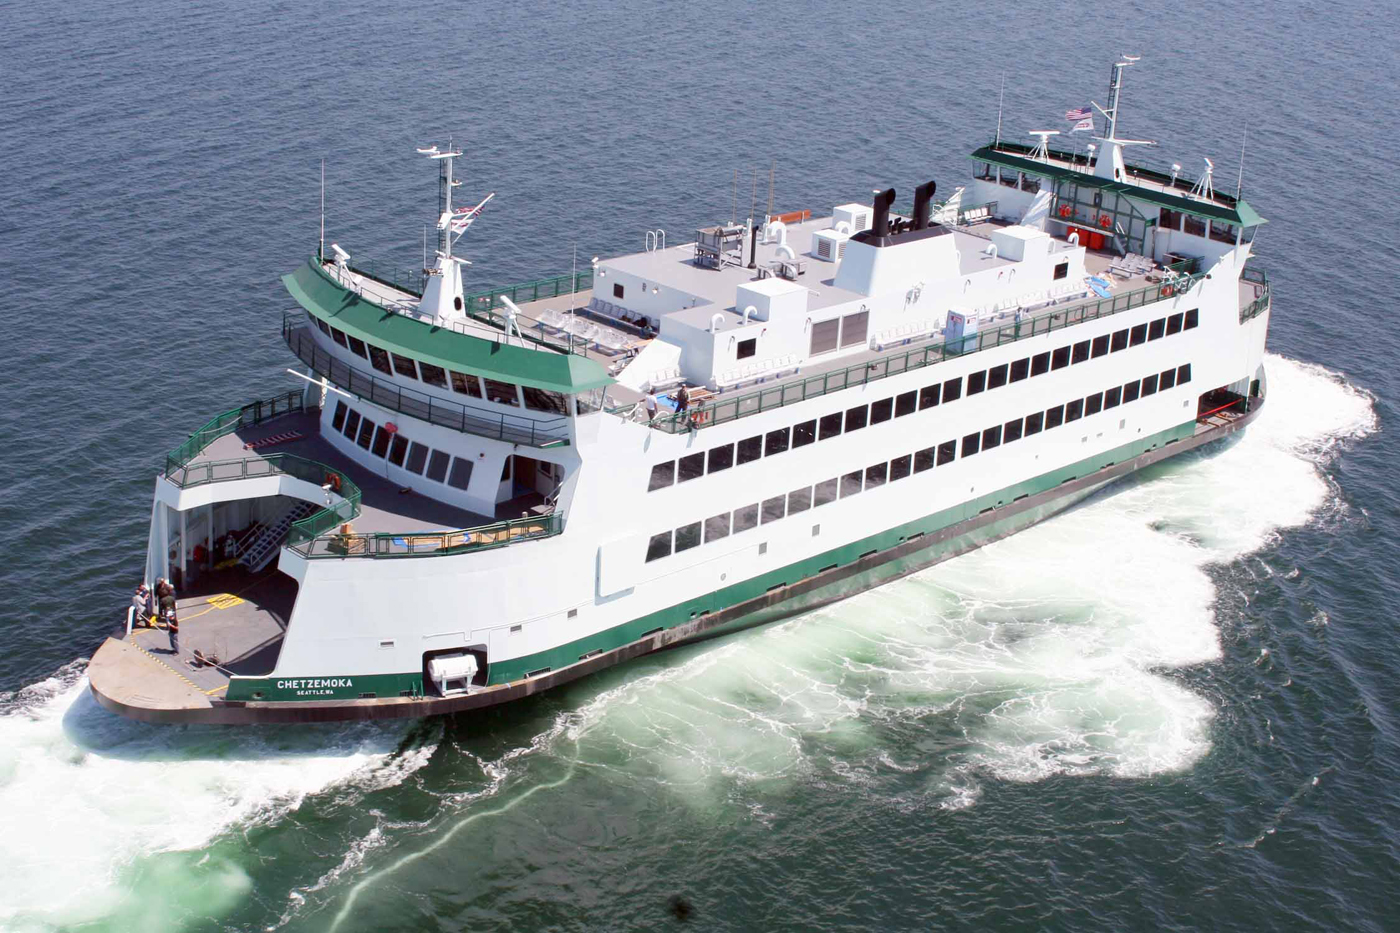
\includegraphics[scale=.15]{images/ferry.jpg}
  \caption{A prototypical WSDOT ferry on its route.}
  \label{fig:basicferry}
\end{figure}

We attempt to predict the tardiness of ferries, defining tardy 
as no less than three minutes later than the initial (at day's beginning) 
scheduled arrival or departure time. We consider both arrival and departure 
times since we predict them separately later on. This definition
of tardiness was chosen to allow for a non-trivial number of tardy events 
(more than 10\% in the data) and to remain practical: i.e. someone could use the
restroom in three minutes time or otherwise make use of that information. The 
Washington State Department of Transportation's ferry system in the Pacific
Northwest served as the source for all data. This system is of 
particular interest for its sheer volume of passengers: 22 million per year 
\cite{wsfTraffic}.  The volume lends itself well to the application of 
data mining techniques. While many techniques exist for data mining and 
prediction in general, support vector machines are used in this project far a 
variety of reasons.


\section{Preliminaries}
\label{sec:prelims}
We consider two approaches popular in terms of both available implementations and 
the literature to be highly applicable to this problem:
artificial neural networks (ANNs) and support vector machines (SVMs). These two 
approaches are algorithms, or machines, for
\textit{supervised learning}: feed labeled (known) data into an
algorithm that learns to make better predictions through comparing its own 
predictions to the labeled data set. Classical examples of using ANNs and SVMs are
spam detection in emails, determining images with cancer present, or even
detecting gender from a facial image. ANNs and SVMs are often considered to be
very similar in the problems they tackle, especially since each can
be used to train a linear classifier: a function taking in some object and 
determining a class to which it belongs. Specifically, a linear classifier uses
a linear combination of the object's features, often represented as a vector and
called a feature vector, to make a classification decision.

Rather than considering tardiness as a 
spectrum of degrees, we approach tardiness as a binary feature: late or not. This 
conceptually simplifies our problem and makes a larger set of ANNs and SVMs 
available for use and adds questions regarding which features are important in 
the ferry system. 
If artificial neural networks and support vector machines 
can both solve classification problems, however, which are we supposed to choose?

\subsection{ANN and SVM}
\label{sec:ann_svm}
Byvatov et al. examine the differences of the two approaches for classifying drugs
\cite{byvatov2003comparison}. While their model certainly isn't for a ferry 
system, their discussion suggests data sets with many features (an aspect of the 
ferry model we discuss later) may be predicted with a smaller standard error by
SVM, albeit only marginally in some cases. Most importantly, they conclude,
along with their references, the two approaches are complementary. Each 
tool yields different false positives (late), false negatives (not-late), true
positives, and true negatives, although SVM may require less ``tweaking''. Even
with such strong similarities, a few reasons exist, leading to the choice of SVMs.

To the non-expert support vector machines are intuitively motivated. Consider 
mapping the
features of a ferry trip (time of departure, weather, boat name, etc.) into a
coordinate plane.  Now, if we do this for all the points in our training set,
we can also attach labels to the points (late or not, as in 
\textbf{Figure~\ref{fig:basic_svm_data}}). In two dimensions, we
could try drawing a line through the late and not-late points to separate them.
This line is simply a hyperplane in higher dimensions, and SVM has its theoretical
underpinnings based on the idea of drawing this hyperplane as an optimal separator. 
Apart from the possible ease of use and understanding, there are also examples of 
SVMs being used in similar traffic prediction systems, providing a baseline 
comparison and the final reason for choosing SVMs over artificial neural networks.

\begin{figure}[h]
  \centering
  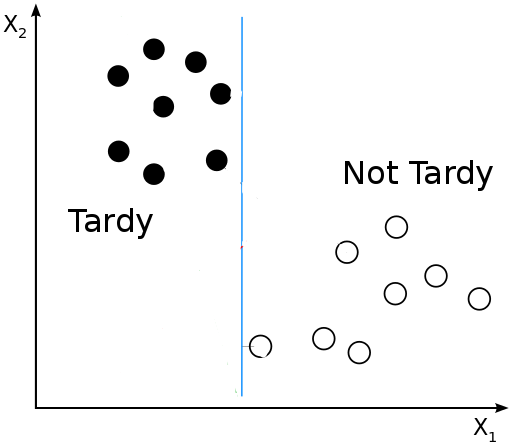
\includegraphics[scale=.5]{images/basic_svm_data.png}
  \caption{A simple example of a separating line for tardiness. 
      Each data point (or instance) has features $X_1$ and $X_2$, corresponding
      to axes on the graph.}
  \label{fig:basic_svm_data}
\end{figure}

Smith et al. use SVM to predict the timeliness of airline
traffic in conjunction with weather patterns \cite{smith2008decision}. Their goal 
is to predict the likelihood of requiring a ``ground delay program'': air traffic
control shuffling flight times
to account for tardiness in the schedule. The model they use involves traffic 
flow management programs to estimate the effects of capacity on an air traffic 
system, and train the SVM on labeled data to produce a function predicting 
the need of a ground delay program and/or an actual delay. Their system was
found to be $78\%$ accurate in predicting need of a ground delay program and $83\%$ 
accurate in predicting a delay. Combined with the discussion in 
\cite{byvatov2003comparison}, it seems that linear classifiers near $80\%$ 
accuracy are within a range of acceptance.

Air traffic and the ferry system are quite alike: exhibiting a
sensitivity to weather, attempt to adhere to a strict schedule, and heavy use.
Due to these similarities, Smith's access to resources like the AMPL supercomputer, 
and his group's expert knowledge, we use $80\%$ as the target accuracy for our
ferry model. Accuracy serves as a crude investigative tool and measure of 
comparison for our first passes, but in \textbf{Section~\ref{sec:beyond_accuracy}}
we investigate the precision and recall of the various linear classifiers our
work yields. These measures weren't discussed in \cite{smith2008decision} but
grant us deeper insight into the usefulness of our work. 

As a final note regarding the usefulness of SVMs, they can be used for regression 
analysis in large
data sets with many variables \cite{chang2011libsvm}. While our project does not
utilize this aspect of SVMs, the possibility of performing such an analysis with the
same tool was one more reason for choosing support vector machines.


\subsection{Basics of SVM}
\label{sec:basics_svm}
A brief overview of the principles behind support vector machines and their use
helps to explain basics of this project. As stated earlier,
SVMs are used to find a linear classifier (some function) for a set of data.  In
this project, we seek a way to separate ferry trips that will be three minutes
past their scheduled time (late) or less (on time). To find the linear classifier,
an SVM uses a feature vector, $F$, to describe ferry trips.  An example $F$ may have
entries for

\[F=\begin{bmatrix}
        EstimatedArrival \\
        BoatName\\
        Temperature\\
        WindSpeed
\end{bmatrix}.\]

This feature vector needs to be entirely numerical, so categorical variables like
boat name must be encoded as numbers.  It is possible to assign boat names to
different values, but most often, the best method expands the feature like a bit
vector.  If there were boat names \textit{SS Minnow, Death Star,} and 
\textit{Millennium Falcon}, then our new $F$ would be

\[F=\begin{bmatrix}
        EstimatedArrival \\
        SS\_Minnow\\
        Death\_Star\\
        Millennium\_Falcon\\
        Temperature\\
        WindSpeed
\end{bmatrix},\]

where the entries for boat names are a $1$ if this trip has that name and $0$
otherwise. Reasons better detailed in \cite{chang2011libsvm} consider this a  
best practice, but suffice it to say that this format is better scaled, and 
leads to superior SVM performance (both in runtime and accuracy).

Along with feature vectors for every trip, an SVM uses a weight vector, $w$,
as the backbone for the linear classifier. Thus, this $w$ is what the
SVM trains. Taking the dot product of $F$ and $w$ determines which class a 
trip's feature vector corresponds to, with negative outputs corresponding to 
late and positive to on time. Moreover, while training on the labeled data
the SVM adjusts $w$ whenever it predicts incorrectly.  The amount to adjust
can vary based on the implementation, but over time $w$ improves on its ability
to predict the class of any instance in the training set.

An optimal solution to $w$ would form a hyperplane separating the instances
perfectly by class. \textbf{Figure~\ref{fig:training_hyperplanes}} illustrates an
example of how an SVM might train a weight vector for a linear classifier 
(represented graphically as
a line) over a set of training data. The final vector, $H_3$, is  
optimal because it maximizes the distance between itself and the nearest points
of each class with no two points of a different class on the same side of the 
line. In the example, we can separate the data with a 
line, but in the real world, and our ferry problem, this rarely works.

\begin{figure}[h]
  \centering
  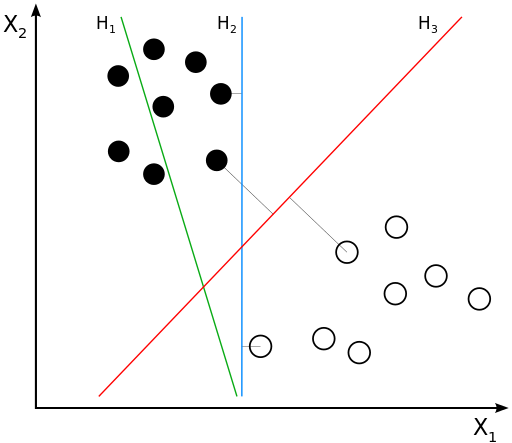
\includegraphics[scale=.5]{images/Svm_separating_hyperplanes.png}
  \caption{As in \textbf{Figure~\ref{fig:basic_svm_data}}, we are trying to separate
    labeled points with a line. An SVM does this iteratively, meaning line $H_1$
    would be the first pass, $H_2$ the result of refitting $w$, and $H_3$ the final 
    classifier produced by the SVM.}
  \label{fig:training_hyperplanes}
\end{figure}

\subsection{Kernel mapping}
\label{sec:kernels}
\textbf{Figure~\ref{fig:kernel-machine}} has an example of data we can't separate.
This exemplifies most real world data: inseparable by a hyperplane. The problem this
creates is that we can no longer look for a linear classifier. A nonlinear 
classifier must be used, a significantly more difficult problem. We might consider 
looking for something within reasonable bounds, since no optimal
hyperplane exists. Difficulty arises in formulating how long an SVM should ``look'' 
for the hyperplane, however. Fortunately, the kernel trick does away with this 
problem through a transformation of the data \cite{aizerman1964theoretical}.

The kernel trick maps the instances of data into a higher dimensional space 
(often much higher), and the SVM works to find a separating plane in the new 
space. The example in \textbf{Figure~\ref{fig:kernel-machine}} gives an idea
of what the mapping would do to the data. The kernel function used in this 
project is a Gaussian radial basis function and was chosen for its popularity
and since the LibSVM library implements it as the default kernel 
\cite{chang2011libsvm} (discussed in the next section). 

\begin{figure}[h]
  \centering
  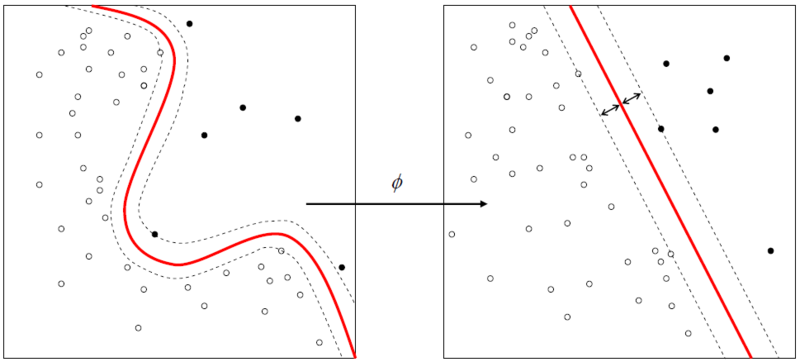
\includegraphics[scale=.6]{images/kernel-machine.png}
  \caption{Separating the data in the first part requires a mapping into an
      often much higher dimension. This mapping makes it possible for a learning 
      algorithm like SVM to find at least some separating hyperplane.}
  \label{fig:kernel-machine}
\end{figure}

Using the kernel trick requires a small addition to the training process. Optimal
parameters for the kernel function need to be found before fitting with the SVM.
An exhaustive grid search performs this task:
\begin{enumerate}
    \item The user supplies a space of parameters to try.
    \item Within this space, create a search grid.
    \item ``Try'' each grid square by using parameters within to transform
        the data and then run the SVM on a subset of the training data.
    \item The best grid square turns into a grid and the process repeats 
        until results stabilize.
\end{enumerate}

So, training the kernel parameters requires training the SVM on very small sets
of data many times to find the best parameters in a space provided by the user.

Implementing all of the functionality of an SVM and kernel function would require
expert knowledge and a thorough amount of validation. There are also concerns 
regarding optimality and an ability to compare results. Fortunately, libraries to 
work with SVMs and kernel functions already exist.

\subsection{LibSVM}
\label{sec:libsvm}
LibSVM \cite{chang2011libsvm} from Chih-Chung Chang and Chih-Jen Lin provides the
implementation of SVMs we used.  This library has bindings to many languages, is 
reasonably straightforward to use from the command-line, is well tested, and has an 
acceptable amount of documentation. In fact, their introduction guide 
\cite{chang2011libsvm} is incredibly helpful both for understanding how SVMs work
and using their implementation. It is also very encouraging that many thousands of
papers cite the LibSVM implementation.  Using this implementation of an 
SVM allowed a great deal of time to be saved and provided a higher degree of 
certainty in the results.

\section{Predicting tardiness through data}
\label{sec:problem}
Before we dig into the details of our data set, let us note a few details regarding
the use of data with an SVM.  Support vector machines require two sets of labeled 
data to find a linear classifier:
training and testing. Feeding the training data into an SVM helps to adjust 
the weight vector for the linear classifier, and the testing data helps 
to check the accuracy of the SVM's product.  These two sets absolutely must 
be disjoint. Otherwise, the SVM basically cheats by being
tested on data it already learned from. There is no clear indicator for how much 
data is needed to successfully train an SVM, but too little means the SVM can't 
generalize and too much can lead to \textit{overfitting}. Overfitting is when an 
SVM trains on too much data of similar qualities so that it fails to accurately
classify data of different qualities. This roughly corresponds to finding patterns
which only apply to a small sample of the real instances, so it often rests 
on the engineer to determine the appropriate amounts of data for training
and testing sets based on experience, experimentation, and availability. Below,
we discuss our decision for these sets, primarily based on having practical
seeming numbers of late and not-late instances in both sets along with the intent
to experiment with various sizes later.

We are now ready to discuss the data used in the analysis and model creation: 
just how much is necessary, where it comes from, the formats, and the ways we
processed it for the SVM training.


\subsection{Washington State's ferries}
\label{sec:wsdot}
The Washington State Department of Transportation (WSDOT) runs the ferry system
in the Pacific Northwest (since 1951) over a stretch of more than 130 miles, from 
Victoria, British Columbia to Point Defiance in Tacoma \cite{wsdotFleet}. The system 
serves over 22 million passengers per year in about $160,000$ sailings 
\cite{wsfTraffic}.  We refer to one sailing (from one terminal to another) as a 
trip.  \textbf{Figure~\ref{fig:ferry_system}} gives the map of the WSDOT's 20 
terminals and 10 routes, lending perspective to the size of the entire system.

One concern during this process is that the ferry system itself as on 
time $95\%$ of the time. It's not clear how this impacts the
practicality of an SVM in this problem nor what reasonable upper and lower bounds
on expected accuracy should be, so the benchmark of $80\%$ from the
airlines paper \cite{smith2008decision} remains the target in this project. The
WSDOT's definition of on-time isn't made clear in their report. Examining the 
data, however, reveals that our definition of on-time leads to approximately
$13\%$ of trips being late. For better or worse, this predictability in the 
system suggests a basic model could call everything not-late and be $87\%$ 
accurate, but the discussion in \textbf{Section~\ref{sec:beyond_accuracy}} 
shows that recall and precision are other important factors we might be able to 
improve on.

\begin{SCfigure}
  \centering
  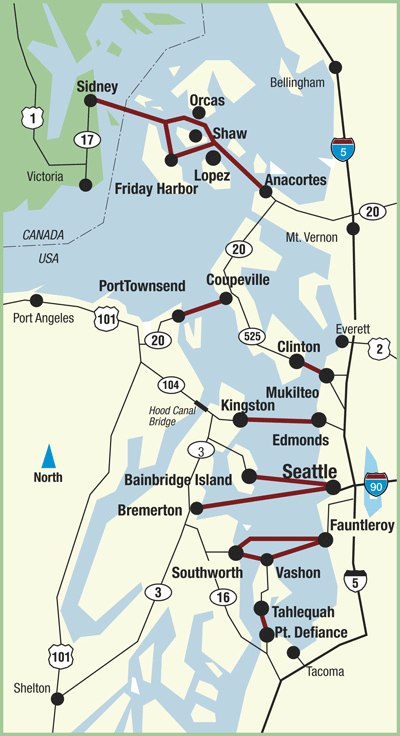
\includegraphics[scale=.4]{images/route-map-overview.png}
  \caption{The Washington State Department of Transportation ferry system. 20
  terminals, making 10 routes, serve users from Point Defiance in Tacoma up to
  Victoria in British Columbia \cite{wsdotVesselWatch}.}
  \label{fig:ferry_system}
\end{SCfigure}

The system stands out for more than just its traffic. Several of the routes
are rather windy looking, suggesting they may be more susceptible to weather and
traffic delays. Some terminals, furthermore, are a hub for several routes. We
might conjecture these terminals to be susceptible to pileups in traffic. These 
and other complexities of the system make the use of a complex SVM model attractive,
and perhaps preferable given the vast data the WSDOT has stockpiled for their
system. 

To effectively use an SVM, we need enough data we can experiment with and it needs
to be in a uniform, accurate state. Originally, a web scraper was written to grab
information from the WSDOT VesselWatch \cite{wsdotVesselWatch} page, but this was 
rendered obsolete when a request for information was fulfilled. The WSDOT 
provided, upon request, a record of
approximately $340,000$ ferry trips from September of 2010 to September of 2012. The
data came as a comma separated value file with the nine fields. See 
\textbf{Figure~\ref{fig:example_wsdot_data}} for an example.

\begin{figure}
    \centering
    \begin{tabular}[h]{lllll}
        \hline
        Vessel & Departing & Arriving & Sched Depart & Actual Depart \\
        \hline
        Kittitas & Mukilteo & Clinton & 9/1/2010 0:00 & 9/1/2010 0:01 \\
        Sealth & Vashon & Southworth & 9/1/2010 0:05 & 9/1/2010 0:06 \\
        Tacoma & Colman & Bainbridge & 9/1/2010 0:15 & 9/1/2010 0:19 \\
    \end{tabular}

    \begin{tabular}[h]{llll}
        \hline
        Initial ETA & Actual Arrival & Date & Route Name\\
        \hline
        9/1/2010 0:13 & 9/1/2010 0:14 & 9/1/2010 & Mukilteo - Clinton \\
        9/1/2010 0:16 & 9/1/2010 0:19 & 9/1/2010 & Southworth - Vashon \\
        9/1/2010 0:45 & 9/1/2010 0:51 & 9/1/2010 & Seattle - Bainbridge Island \\
    \end{tabular}
    \caption{The header of the data provided from the WSDOT along with the first
        three lines (broken into two tables
        to fit page widths). There are over $340,000$ lines in the original file.}
    \label{fig:example_wsdot_data}
\end{figure}

The column headings are all fairly straightforward, but the
scheduled and initial values, for departure and arrival respectively, are the
times found on the schedule for the beginning of the day. We didn't expect to 
have both predicted and actual times for both arrivals and departures, so the
problem was reformulated to apply to tardiness for either type of scheduled
time. To account for this, we separate the table in two: one for
data pertaining to arrivals and one for departures. The arrival table actually 
includes the departure information since this is still pertinent to predicting
the arrival time (an apparently easier problem with this information, which we
discuss in \textbf{Section~\ref{sec:gen_results}}). The two tables essentially
give us two data sets and two problems: predicting arrival tardiness and predicting 
departure tardiness.

Before feeding the data into the SVM, it was necessary to transform times and 
categorical variables into numeric values. This was done through several Python
scripts: using seconds past January 1, 1970 for the times and expanding the 
categoricals out as many variables functioning like a bit vector (addressed in 
\textbf{Section~\ref{sec:basics_svm}}). Additionally,
and a far more difficult problem, we joined this ferry data with weather data
obtained from the National Oceanic and Atmospheric Administration (NOAA).

%       and manage to set the stage for how this research impacts people
%  A portrait of the system</h2>
%       Established in 1951</li>
%        22 million passengers per year</li>
%        20 terminals, 10 routes, 23 vessels</li>
%        Largest ferry system in the world for vehicles</li>
%        From Victoria to Pt. Defiance (~130 miles)</li>
%        159,811 sailings in 2012 (12,764 in December)</li>
%        Almost 10,000,000 vehicles in 2011</li>
%     <img width="110%" 
%      src="images/route-map-overview.gif" align="right">
%  Go over the details of the ferry system.
%  1. history
%  1. Boats
%  2. # Of trips per day
%  3. Routes
%  4. Places serviced
%  6. Design and planning
%  7. Resources for travelers
%    1. Vessel Watch
%    2. Pamphlets
%    3. General knowledge
%    4. Email alerts
%  * Mention that ~95% of boats are on time.  This poses some interesting
%    questions about what we can actually learn.
% 
%  96.4% on time 
%  Best: Pt. Defiance/Tahlequah and Edmonds/Kingston (99.5%)
%  Worst: Anacortes/San Juans (88.9%)
% 

\subsection{Weather and final SVM format}
\label{sec:data_origins}
Retrieving accurate and full historical weather data presented an unexpected 
challenge. Most weather sites are focused on future weather and make historical
data available only through programming APIs which may require a paid subscription.
Fortunately, NOAA provides (by a subscription our institution already has) a portal 
for retrieving weather data
by station. Stations record over $20$ different features at some point every hour.
It seems that some stations experience outages or are unable to record on some
instruments every so often; because of this, we used the station with the seemingly
most complete data set in the area. This turned out to be a station near the 
Tacoma Narrows Bridge. The data was downloaded in files by month for the range of
September 2010 to September 2012 from a quality controlled store on NOAA's 
site \cite{noaaWeather}. Only about $1,000$ of the more than $24,000$ weather 
entries had to be removed for null entries.  Unfortunately, 
the station is not a central point, but it seemed close enough at the time. 

In \textbf{Figure~\ref{fig:weatherExampleLine}} is an example of the weather
data in its raw form. Note there are some categorical variables, but
nearly everything is a numeric. The categorical variables weren't utilized in the
final model, since they can be inferred from the other data. Many of the columns
are simply blank, due to the stations lack of equipment for certain measures. 
The measures for dry bulb, wet bulb, dew point, wind speed, wind direction, and
station pressure were used in the final model. There was very little missing data
for any of these, and none of them directly imply another. Humidity may seem to 
be missing, but it can be calculated by the dry bulb and wet bulb temperatures.

We avoided using multiple stations to keep the joining of ferry and weather 
data simpler: since all ferries matched with one station, we just found the 
weather recording closest (within at least an hour) of the actual time reported
on the ferry trip. Of the over $340,000$ ferry trips, only about $13,000$ had to 
be removed for lack of weather data.  With a data set so large, this only 
constituted $4\%$, an acceptable loss in our case. To join the data, a simple
Python script searched the weather data for a nearest time to join with each
ferry trip, and then the departure and arrival information were separated to
place each as an individual event in separate files. It was then straightforward
to calculate the label (late or not) for each event by subtracting the appropriate
times.

\begin{figure}
    \centering
     \begin{tabular}{llll}
        WBAN & Date & Time & StationType \\
        SkyCondition & SkyConditionFlag & Visibility & VisibilityFlag \\
        WeatherType & WeatherTypeFlag & DryBulbFarenheit & DryBulbFarenheitFlag \\
        DryBulbCelsius & DryBulbCelsiusFlag & WetBulbFarenheit & WetBulbFarenheitFlag \\
        WetBulbCelsius & WetBulbCelsiusFlag & DewPointFarenheit & DewPointFarenheitFlag \\
        DewPointCelsius & DewPointCelsiusFlag & RelativeHumidity & RelativeHumidityFlag \\
        WindSpeed & WindSpeedFlag & WindDirection & WindDirectionFlag \\
        ValueForWindCharacter & ValueForWindCharacterFlag & StationPressure & StationPressureFlag \\
        PressureTendency & PressureTendencyFlag & PressureChange & PressureChangeFlag \\
        SeaLevelPressure & SeaLevelPressureFlag & RecordType & RecordTypeFlag \\
        HourlyPrecip & HourlyPrecipFlag & Altimeter & AltimeterFlag
    \end{tabular}


        \[94274,20110101,0053,12,CLR, ,10.00, , , ,25, ,-3.9, ,22, ,-5.4, ,\]
        \[16, ,-8.9, , 69, , 0, ,000, , , ,29.69, ,1, ,002, ,30.04, ,AA, , ,\]
        \[,30.03, \]

    \caption{An example line from a weather data file preceded by the many, but 
    thankfully explicit, column headings.}
    \label{fig:weatherExampleLine}
\end{figure}

Following the joining of weather and ferry data and the labeling, it is necessary to
scale the data between $-1$ and $1$, an SVM best practice
to make no feature stand out by sheer magnitude \cite{chang2011libsvm}. LibSVM 
performs this transformation quickly and is also useful for separating out the 
training data from the testing data. We used it to randomly sample about 
$270,000$ data points for training and $50,000$ for testing. The sampling 
was random to the extent that both sets of data contained a roughly equal 
distribution of late and not-late ferry trips. This is an incredibly important
feature to preserve, since we want to both learn about tardiness and check if the
linear classifier produced predicts both scenarios. We stated earlier that
it was unknown what amount of data to train on, so the size of the training set
here was chosen as a baseline to be examined and experimented with should time 
permit. With separated data in hand, we proceeded to train a linear classifier 
using the LibSVM package.


\section{Results}
\label{sec:results}
The modeling aspect of the project took place in roughly three phases. As 
described before, the primary goal models the ferry system and answers the 
question of whether or not using an SVM to train a linear classifier proves useful 
for ferry traffic. This leads to the first two phases
which involve a first pass and then a serious refining of the methodology.  Recall 
that we consider approximately $80\%$ accurate on the test data to be comparable
with Smith et al \cite{smith2008decision}, since like that group, we wish to see
if using SVM is a practical method for determining ferry tardiness. 
A secondary goal is to find which features matter in determining tardiness.  While
this goal asks questions best answered by a regression analysis, we 
attempt a crude approximation through empirical methods.  The final component is 
a small experiment to test interesting phenomena arising in the general results.  
This latter part may be the most interesting of the project, but we begin 
first with an attempt to use LibSVM.

\subsection{The first pass}
\label{sec:firstpass}
We first tried determining whether or not a ferry is on
time for its departure, leaving arrival for after the process was worked out. 
A file with all of the labeled training instances was fed into LibSVM, using the
default parameters of the kernel. The process took an entire night running on
low end hardware, and the results were disappointing to say the least.

After running on the test data, the linear classifier only yielded $60\%$ accuracy. 
This is significantly beneath the benchmark. The time to run the process was also
surprising and led to a more cautious approach for the rest of the work. It became
clear at this point how precious each run would be (for time and computing 
resources). 

To 
improve the performance of the classifier, LibSVM provides an exhaustive guide 
\cite{chang2011libsvm} for beginners in the perils of simply ``running it''. The 
directions weren't followed on the first pass because it was hoped the process 
would be much simpler just using the default parameters. Although this approach
was wrong, it provides anecdotal evidence regarding the importance of being 
thorough and following the steps in the guide.

Having learned some lessons, the LibSVM guide was followed to the letter on a 
second pass. The only major change to the process was training on the 
parameters for the kernel function. As mentioned before LibSVM provides code
to perform an exhaustive search for the best fit parameters to use in the function.
The subsets for this training come from the training data. Finding the best fit 
parameters is a long process, sometimes as long as the actual SVM training, so it
slows down the process significantly, but as we're about to discuss the results
are well worth it.

\subsection{General results}
\label{sec:gen_results}
Training the SVM to predict arrival time tardiness proved to be the most successful.
In this case, a full trip description (feature vector) included features for the 
actual departure 
time, all weather, predicted arrival time, date, vessel name, departure location, 
and arrival location. (Final results for all runs are displayed in 
\textbf{Figure~\ref{fig:second_run_data_arrivals}}.) We expect for this to 
be the problem the SVM can be most accurate about, since really it only needs to 
understand how long the trip takes a ferry. 

The tardiness of full feature instances were able to be predicted with 
$\approx 87.0\%$ accuracy. For a second pass, this is fantastic to be above the
benchmark of $80\%$. Given that about $87\%$ of trips are on time though, this 
accuracy shouldn't be surprising. In fact, we could achieve the same results 
by guessing all trips are on time, so this model isn't as exciting as we might
like. We'll examine more ways to check the usefulness of the model in 
\textbf{Section~\ref{sec:beyond_accuracy}}. 

To tune the linear classifier from our SVM, we should
try trimming unnecessary features to find maximum accuracy. Due to time 
constraints, the trimming we perform here is very coarse. A thorough examination
would attempt to examine all combinations of features, but this is beyond the
scope of our work, especially in regards to available computing power.

Removing the departure information from the features drops accuracy to $60\%$, 
a disappointing result. It may be possible to dramatically improve this result with
some of the techniques discussed in \textbf{Section~\ref{sec:improvements}}.
To determine whether removing more features made any significant difference, we
also removed the weather information from predicting arrivals, yielding 
the more interesting result which we discuss after departure prediction.

\begin{figure}
    \centering
    \textbf{Arrival Predictions}

    \begin{tabular}{ll}
        Configuration & Percent accuracy on test data\\
        Full          & $87\%$\\
        No Departure  & $60\%$\\
        No Weather    & $88\%$\\
        No Departure, No Weather  & $59.4\%$\\
    \end{tabular}
    \caption{Feature configurations and their associated percent accuracies in
         predicting the timeliness of arrivals convey the empirical importance of 
         the features included.}
    \label{fig:second_run_data_arrivals}
\end{figure}

A full departure trip description includes all of the information regarding a trip
(vessel name, estimated time of departure, route) and the weather. 
The prediction results here were not
as exciting as with arrivals, but they proved to be more stable. The full 
departure vectors were predicted with $76.3\%$ accuracy, and removing weather
only reduced accuracy to $75.7\%$. While $76\%$ is not at the benchmark, having
experienced the change removing features and adjusting the training sets can have,
it seems like more time with the data could yield even better results.

When departure information is still included in arrival predictions, the removal of 
weather actually improves accuracy resulting in $88\%$, an improvement of one
percentage point. Without the departure information, the percent accuracy decreases
by only $0.6$ percentage points, a negligible difference at $59.4\%$ accuracy. 
Weather was included as all but a given for improving the accuracy of the SVM
work, but the results just outlined call into question this assumption and 
warranted further investigation.

\begin{figure}
    \centering
    \textbf{Departure Prediction Accuracy}

    \begin{tabular}{ll}
        Configuration & Percent accuracy on test data\\
        Full        & $76.3\%$\\
        No Weather  & $75.7\%$\\
    \end{tabular}
    \caption{Feature configurations and their associated percent accuracies in
         predicting the timeliness of departures convey the empirical importance of 
         the features included.}
    \label{fig:second_run_data_departures}
\end{figure}

\subsection{The problem with weather}
\label{sec:weather_prob}
Since weather made barely any difference in prediction accuracy (even 
degrading it in some cases), examining possible causes of this unexpected 
incident became the last focus of the project. By re-examining the assumptions
made regarding weather at the start, there are several which we can now dispute:

\begin{enumerate}
    \item Weather helps improve accuracy.
    \item \label{wAssumption_oneStation} The area is geographically small enough 
        that one weather station should be just fine for all routes.
    \item The weather variables dry bulb, wet bulb, dew point, wind speed, 
        wind direction, and station pressure are the right variables to examine.
    \item The data retrieved is of a sufficient quality.
\end{enumerate}

Given time constraints and the results of the SVM, it seems assumption 
\ref{wAssumption_oneStation} is the best to tackle. But what how can we tease
apart this assumption? Our strategy was to tackle the effect of the station
location by comparing the effect of weather on three routes sufficiently far apart.
Running individual SVMs for each route (testing accuracy only on that route's 
trips). The three routes chosen were Tahlequah-Point Defiance, Kingston-Edmonds,
and Coupeville-Port Townsend. Looking at \textbf{Figure~\ref{fig:ferry_system}},
we can see the furthest route, Coupeville-Port Townsend, is nearly $100$ miles
from the weather station near Point Defiance. These three were deemed to be 
closest, middlemost, and furthest from the weather station, respectively, but also 
have enough trips to warrant an individual SVM. 

The results of the experiment are mixed and can be viewed in full with 
\textbf{Figure~\ref{fig:weatherExperiment}}. We used the full feature vectors 
(described in \textbf{Section~\ref{sec:gen_results}}) for 
predicting both arrivals and departures, only taking out weather where noted
for the comparison. We can see that the removal of weather rarely made a difference
in any of the measures, except for the Kingston-Edmonds route when looking at 
arrivals. In that case the removal of weather was a major boon the accuracy. 
Otherwise, the results here are inconclusive of the actual efficacy of weather
in improving predictions, and if anything, only help confuse the situation.

\begin{figure}
    \centering
    \textbf{Prediction accuracies with a $Weather/NoWeather$ format}

    \begin{tabular}{ll}
        \textbf{Arrivals} & \textbf{Departures}\\
        \hline
        Tahlequah-Point Defiance    & \\
        95.2\%/93.9\% & 76.1\%/75.3\% \\
        Kingston-Edmonds    & \\
        85.2\%/94.7\% & 82.7\%/82.8\% \\
        Coupeville-Port Townsend     & \\
        88.3\%/87.7\% & 68.8\%/69.4\% 
    \end{tabular}
    \caption{The arrival and departure time prediction accuracies for individual 
        routes when including and excluding weather.}
    \label{fig:weatherExperiment}
\end{figure}

The robustness of the ferry system provides another possible explanation. Recall 
we that
our definition leads to only about $13\%$ of ferry trips being late, a remarkable 
feat for the WSDOT. It may simply be that there isn't much of a pattern in regards
to weather or other predictable phenomena. We may be looking at a system whose
only fault is vessel maintenance, a feature requiring very different data than
that which we had access to. 

The accuracy of the linear classifiers produced by our SVM runs are promising,
but so far we have used accuracy as the only measure of effectiveness. We now 
turn our attention to confusion matrices, precision, and recall. These features
allow us to more thoroughly analyze the first linear classifiers we produced.

\subsection{Beyond accuracy}
\label{sec:beyond_accuracy}
As mentioned before, accuracy is only a crude measure of success. It also binds us
to comparing our models with a ``naive'' model which always guesses not-late and
is $87\%$ accurate. Investigating the precision and recall of our models each other,
with more than accuracy, reveal the nuances of prediction \cite{classifierEval}. 
We use confusion matrices to visualize the results and help calculate the 
precision and recall. A confusion matrix displays the actual classes against 
the predicted classes to convey the true positive (late), true negative 
(not-late), false positive, and false negative results:

\begin{center}
\begin{tabular}[h]{l|ll}
                     & actual class &  \\
     \hline
     predicted class & True Positive ($tp$)& False Positive($fp$)\\
                     & False Negative ($fn$)& True Negative($tn$)\\
\end{tabular}
\end{center}

Here we are considering positive to mean a trip flagged as 
late and negative as not-late. The diagonal of the matrix tells us the trips our
classifier correctly predicts, and non-zero values off the diagonal indicate 
incorrect classifications. Thus, we calculate precision by

\[Precision=\frac{tp}{tp+fp}\]

and recall with

\[Recall=\frac{tp}{tp+fn}.\]

Higher precision corresponds to an ability to return \textit{more relevant results 
than irrelevant results}, and high recall means an algorithm returns \textit{most of
the relevant results}.  So with high precision, a trip flagged as late is more 
likely to be late than not-late. High recall means our model catches most of
the late trips. These two measures go beyond just accuracy and tell us more about
the usefulness of our model.

First note we are using the testing sets to find this data, so the number of 
trips we are considering is $50,000$. Also, a perfect score for either recall or
precision is 1. It's incredibly unlikely, and probably unreasonable, to expect 
such a score. In fact, the only reasonable scenario for this would be with an
entirely deterministic system.  We now look at scores for the weather/no-weather 
models of arrival
departure tardiness from \textbf{Section~\ref{sec:gen_results}}. This examination
hopefully makes clear the differences beyond accuracy.

We start by examining the arrivals with departure information. Recall the 
classifier is $87\%$ accurate with weather and $88\%$ without, as good as the
naive model just discussed, but we consider this model to have an 
``unfair advantage'' by knowing information about departures. 
\textbf{Figure~\ref{fig:confusion_arrivals}} displays this model's confusion
matrix.
The high accuracy of this model reveals itself in the low numbers off of the 
diagonals, but the precision and recall are what we hope differentiates
this model from naive guessing. 

% Full/NoWeather: high accuracy with departures 
% 87 weather/ 88 no weather
\begin{figure}
    \textbf{Arrivals}

    \begin{tabular}[h]{l|ll}
                         & actual class &  \\
         \hline
         predicted class & $17,574 $ ($tp$)& $1,974$ ($fp$)\\
                         & $4,477$ ($fn$)& $25,975$ ($tn$)\\
    \end{tabular}

    \textbf{Arrivals without weather}

    \begin{tabular}[h]{l|ll}
                         & actual class &  \\
         \hline
         predicted class & $18,122$ ($tp$)& $2,115$ ($fp$)\\
                         & $3,878$ ($fn$)& $25,885$ ($tn$)\\
    \end{tabular}
    \caption{The confusion matrices for predicting arrival tardiness with
    the departure information.}
    \label{fig:confusion_arrivals}
\end{figure}

\begin{figure}
    \begin{tabular}{l|l}
         Classifier & Precision\\
         \hline
         Arrivals & 0.899\\
         Arrivals without weather & 0.895\\
         \hline
         & Recall\\
         \hline
         Arrivals & 0.797\\
         Arrivals without weather & 0.824\\
    \end{tabular}
    \caption{Precision and recall for the arrivals model with departure 
    information.}
    \label{fig:pr_arrivals}
\end{figure}

In \textbf{Figure~\ref{fig:pr_arrivals}}, note the very high precision and recall 
for both the models with and without weather.  The high precision indicates this
model returns substantially more late trips as late than falsely identifying
not-late trips. The high recall also suggests our model returns most of
the late results as late. These are good results, but it remains that this
model requires the departure information, something a user might not have if they
look for a prediction before the departure information becomes available. So, let
us turn to the arrivals model without departure information.

The arrivals model without departure information achieved $60\%$ accuracy with
weather and $59.4\%$ without.  These are significantly lower accuracies than
our model with departure information, but it's possible the precision and recall
values for the model make it competitive in some sense. (Especially since it can
be used long before the departure information becomes available to a user.)
\textbf{Figure~\ref{fig:confusion_arrivals_nod}} contains the confusion matrix 
for this arrivals model.

% 60 weather/ 59.4 without
% Arrival 2: low accuracy without departure info
\begin{figure}
    \textbf{Arrivals without departures}

    \begin{tabular}[h]{l|ll}
                         & actual class &  \\
         \hline
         predicted class & $6,146$ ($tp$)& $4,692$ ($fp$)\\
                         & $15,905$ ($fn$)& $23,257$ ($tn$)\\
    \end{tabular}

    \textbf{Arrivals without departures and weather}

    \begin{tabular}[h]{l|ll}
                         & actual class &  \\
         \hline
         predicted class & $8,696$ ($tp$)& $6,969$ ($fp$)\\
                         & $13,355$ ($fn$)& $20,980$ ($tn$)\\
    \end{tabular}
    \caption{The confusion matrices for predicting arrival tardiness without
    the departure information.}
    \label{fig:confusion_arrivals_nod}
\end{figure}

The lower accuracy of this model comes through in the high numbers off of the 
diagonals.  Otherwise, there isn't anything immediately noteworthy regarding this
model. Neither the true negatives nor true positives stand out as high, so the
model probably isn't better at classifying late events or classifying not-late
events. What can we learn from the precision and recall though? For this 
information, we look to \textbf{Figure~\ref{fig:pr_arrivals_nod}}.

\begin{figure}
    \begin{tabular}{l|l}
         Classifier & Precision\\
         \hline
         Arrivals without departures & 0.588\\
         Arrivals without departures and weather & 0.555\\
         \hline
          & Recall\\
         \hline
         Arrivals without departures & 0.279\\
         Arrivals without departures and weather& 0.394\\
    \end{tabular}
    \caption{Precision and recall for the arrivals model without departure 
    information.}
    \label{fig:pr_arrivals_nod}
\end{figure}

This time, the scores are significantly lower, expected given the low accuracy
of this model. The precisions are almost at $50\%$, indicating the model is
confusing not-late and late events. Additionally, the recalls are below 
$50\%$, meaning a large number of late events are being missed. The low recall
is most troubling: users would be expecting many boats to be late when
they aren't. In a way, this model isn't aggressive enough. The fact that 
the model without weather has a significantly higher recall is interesting. 
Weather continues to yield bizarre effects, possibly suggesting weather
information confuses the ability to pick out late events. This is definitely
worthy of further investigation, but with scores so low we can label this 
model defunct and requiring significant further work.  We still have the 
departures model, however, for which the confusion matrix sits in
\textbf{Figure~\ref{fig:confusion_departures}}.

% Now for departures

\begin{figure}
    \textbf{Departures}

    \begin{tabular}[h]{l|ll}
                         & actual class &  \\
         \hline
         predicted class & $1,466$ ($tp$)& $993$ ($fp$)\\
                         & $10,853$ ($fn$)& $36,688$ ($tn$)\\
    \end{tabular}

    \textbf{Departures without weather}

    \begin{tabular}[h]{l|ll}
                         & actual class &  \\
         \hline
         predicted class & $158$ ($tp$)& $445$ ($fp$)\\
                         & $12,161$ ($fn$)& $37,236$ ($tn$)\\
    \end{tabular}
    \caption{The confusion matrices for predicting departure tardiness.}
    \label{fig:confusion_departures}
\end{figure}

We can see the classifier for departures without weather predicts quite 
a few more trips 
as not-late. Remembering that the departure classifier with weather is $76.3\%$ 
accurate and the classifier without weather is $75.7\%$ accurate, perhaps the
weather information is only good for the relatively small number of trips that 
are actually late. Having investigated the other confusion matrices, this seems
like a possible link: weather is important only for the ``rare'' late cases. 
It's an interesting idea for later study. For now, we turn to the precision and
recall values of the model in \textbf{Figure~\ref{fig:pr_departures}}.

\begin{figure}
    \begin{tabular}{l|l}
         Classifier & Precision\\
         \hline
         Full departure & 0.597\\
         Departure without weather & 0.262\\
         \hline
         & Recall\\
         \hline
         Full departure & 0.119\\
         Departure without weather & 0.013\\
    \end{tabular}
    \caption{Precision and recall for the departure model.}
    \label{fig:pr_departures}
\end{figure}

We can see the full departure classifier actually scores much higher in
both precision and recall. The recall score means the classifier flags about 
$12\%$ of late trips, and the approximately $60\%$ precision means the classifier
flags mostly late trips as late, rather than indicating many not-late trips
as late. The recall suggests we may be missing some indicator of what makes a 
trip late. In the case of precision, the number is encouraging, indicating we 
aren't confusing late and not-late trips, for the most part. The numbers are so
much lower than for arrivals though, even our low accuracy model without departure
information, this departure model isn't looking quite as good. Such a low 
recall means a user of this model might feel like the application is always 
guessing not-late. Obviously, this model needs further tuning.

To tune these parameters, we could try any number of approaches (many outlined in
\textbf{Section~\ref{sec:improvements}}). The arrival models are much more 
interesting than their accuracy indicates, especially given how low the 
departures model scores. After tweaking and testing more, we might find the
arrivals are generally more predictable than departures or there just isn't
a way to consistently classify those fringe tardy trips. Regardless, the first
pass at these models is encouraging.


\section{Closing thoughts}
\label{sec:summary}
We met the original goal of the project, to develop a ferry system model using AI 
techniques, and further investigated the behavior of the
system. We beat the initial benchmark of $80\%$ accuracy for a linear classifier 
produced by an SVM, and we concluded the performance could probably be improved
on given more time and experience tuning the process. The exploration of weather's
relationship to the ferry system also proved to be more complex than expected, 
clouding the assumption of there being a significant link between the two. We 
also examined the precision and recall, discovering mixed results between the 
models. Our most effective model, which had the advantage of departure information,
exhibited high precision and recall, indicating it may be worth further study
as an improvement upon the naive guess of always not-late. The remaining 
questions and further work are now even greater in scope than when the 
project began.

\subsection{Improvements to the data analysis}
\label{sec:improvements}
Most of the percent accuracies we have analysed were short of the $80\%$ benchmark,
but some were very close. More time to tune the features used in prediction, 
check the data quality, and experiment with different training set sizes would
likely yield even better predictions. The latter goal is of particular interest.
Since no definitive guide to using SVM was found before finishing the project, 
the size of training sets was kept the same throughout bet may be a poorly informed
choice. A common criticism of SVMs, and AI in general, is that training on too
large of a dataset can lead to overfitting without realising it. This means the
machine only accurately predicts events similar to the training data
and can't generalize beyond. With a chance to train on smaller sets of data,
we might find overfitting hampers the accuracy we found with larger training sets.

Recall the variance found among training an SVM over individual routes in the 
weather investigation. We discovered that individual routes varied widely, 
suggesting a 
``master'' SVM for all routes may not be appropriate. We would like to assume that
an SVM could tease apart the relationships between routes and tardiness, but there
may be too many conflicts between routes in terms of which features matter. For 
instance, a short route between Clinton and Mukilteo covers mostly open water
and might not be very susceptible to weather in comparison to the island crowded
route from Anacortes to Lopez. A thorough comparison of how individual SVMs 
perform for the routes might make this approach even more appealing or lend 
insight into a better choice.


\subsection{Extensions}
\label{sec:extensions}
The end product of our SVM trainings worked in the ways we hoped: seeming to be 
useful for predicting ferry timeliness and as an investigative tool for the
WSDOT ferry system. Still, the project is far from complete. 

The SVM training produced useful linear classifiers, but a framework for average
users could still be built. Whether this would be a web or mobile application is
unfortunately restricted by the use of LibSVM. Since the only implementation is in 
C, a web application querying some server seems like the most straightforward
approach. There are other possibilities since LibSVM has bindings in many languages,
but the production of a real user interface and seeing it used would certainly 
validate the usefulness of predicting ferry times.

The SVM training itself could also be restructured. Several times, the lack of
production time inhibited the ability to fully explore the data, but beyond this
we could improve the definition of tardy. A multiclass SVM allows us to have degrees
of tardiness (e.g. three minutes, five minutes, or ten minutes late). LibSVM 
supports this sort of SVM, a fairly natural extension of the two class case.
Moreover, LibSVM could be used for a regression analysis of the features. This might
be the best way to determine which features matter in regards to tardiness. 
 
\subsection{Conclusion}
\label{sec:conclusion}
The use of an SVM for predicting ferry times novelly makes use of the large data 
sets available. This tool from artificial intelligence enables us to predict, with
over $75\%$ accuracy in most cases, the tardiness of ferries in the complex system,
and it brings us insight into how important various features are when predicting
this tardiness. While we may not fully understand the strange behavior exhibited
by including weather in the model, the base assumption of weather's importance no 
longer appears valid. Further tuning of the SVM process may yield even
greater insight and perhaps better prediction results. In general, however, the 
results of the project are promising and suggest support vector machines are
a useful approach to modeling the ferry system.

\newpage 

\bibliographystyle{amsalpha}
\bibliography{undergraduate-thesis.bib}

\end{document}












